\section{Experiments}
\label{experiments} 

\subsection{Experimental Settings}
\noindent \textbf{Datasets.} 
We conduct experiments on four widely used long-tailed benchmarks: ImageNet-LT~\cite{liu2019large}, Places365-LT~\cite{liu2019large}, iNaturalist2018~\cite{van2018inaturalist}, and CIFAR100-LT~\cite{cao2019learning}.
ImageNet-LT contains 115.8K images from 1,000 classes, with per-class samples ranging from 5 to 1,280. Places365-LT includes 62.5K images across 365 categories, each containing 5–4,980 images. iNaturalist2018 consists of 437.5K images from 8,142 species, exhibiting a distribution from 2 to 1,000 images per class. CIFAR100-LT is a synthetic long-tailed version of CIFAR100 constructed with imbalance ratios (IR) of 100, 50, and 10.

% \vspace{0.5em}

\noindent \textbf{Metrics.}
Following the protocol of~\cite{liu2019large}, we evaluate all methods on a balanced test set and report the top-1 classification accuracy for three splits: Many-shot (more than 100 samples), Medium-shot (20 to 100 samples), and Few-shot (fewer than 20 samples), as well as the overall accuracy across all classes.

% \vspace{0.5em}

\noindent \textbf{Baselines.}
We compare our method with recent CLIP-based long-tailed recognition approaches, including LiVT~\cite{xu2023learning}, LPT~\cite{dong2023lpt}, VL-LTR~\cite{tian2022vl}, RAC~\cite{long2022retrieval}, BALLAD~\cite{ma2021simple}, and LIFT~\cite{shi2024long}. Following their standard setups, we ensure a fair comparison. Notably, VL-LTR and RAC leverage additional  data sources.

% \vspace{0.5em}

\noindent \textbf{Implementation Details.}
Unless otherwise specified, we adopt CLIP-ViT-B/16 as the backbone and employ AdaptFormer~\cite{chen2022adaptformer} for parameter-efficient fine-tuning. The number of CLIP-selected samples is fixed at $k=5$ for all comparisons.
% , while results under other $k$ settings are provided in the Appendix~\textcolor[HTML]{367DBD}{C}.
We use SGD with a learning rate of 0.01, momentum of 0.9, weight decay of $5\times10^{-4}$, batch size of 128, and a cosine learning rate schedule. All models are implemented in PyTorch and trained on a single NVIDIA GeForce RTX 5090 GPU.

% We conduct experiments on four long-tailed benchmark datasets, including ImageNet-LT~\cite{liu2019large}, Places365-LT~\cite{liu2019large}, Naturalist2018~\cite{van2018inaturalist}, and CIFAR100-LT~\cite{cao2019learning}. 
% ImageNet-LT contains 115.8K images from 1,000 classes, where the number of samples per class ranges from 5 to 1,280. Places-LT includes 62.5K images from 365 categories, with each class having between 5 and 4,980 images. iNaturalist2018 consists of 437.5K images from 8,142 species, with a long-tailed distribution ranging from 2 to 1,000 images per class. CIFAR100-LT is a synthetic long-tailed variant of CIFAR100 constructed with different imbalance ratios (IR) of 100, 50, and 10. Following the protocol of~\cite{liu2019large}, we report the top-1 accuracy on three splits: \textit{Many-shot} (classes with more than 100 images), \textit{Medium-shot} (20–100 images), and \textit{Few-shot} (fewer than 20 images), in addition to the overall accuracy on the entire dataset. 

% For a fair comparison, we follow the standard experimental setup of recent CLIP-based long-tailed recognition methods, including LiVT~\cite{xu2023learning}, LPT~\cite{dong2023lpt}, VL-LTR~\cite{tian2022vl}, RAC~\cite{long2022retrieval}, BALLAD~\cite{ma2021simple}, and LIFT~\cite{shi2024long}. 
% Unless otherwise specified, we adopt CLIP-ViT-B/16 as the backbone and employ the AdaptFormer~\cite{chen2022adaptformer} for parameter-efficient fine-tuning. We fix the CLIP number of samples selected $k=5$ in all comparisons for fairness. We use the SGD optimizer with a learning rate of $0.01$, weight decay of $5\times10^{-4}$, a batch size of 128, momentum of $0.9$ and a cosine learning rate schedule. All models are implemented in PyTorch and trained on n a single NVIDIA GeForce RTX 5090.


\subsection{Comparison with State-of-the-art Methods}
\begin{table*}[!t]
\centering
\caption{Results on CIFAR100-LT comparing different \textit{Finetuning}-based methods under varying imbalance ratios. \textbf{Bold} indicates the best results. * marks reproduced results because the original paper did not report them completely.}
\label{tab:cifar100}
\footnotesize
\begin{tabular}{l|c|cccc|cccc|cccc}
\toprule
\multirow{2}{*}{\textbf{Method}} & \multirow{2}{*}{\textbf{Param.}} 
& \multicolumn{4}{c|}{\textbf{CIFAR100-IR100}}                                    
& \multicolumn{4}{c|}{\textbf{CIFAR100-IR50}}                                      
& \multicolumn{4}{c}{\textbf{CIFAR100-IR10}}                                    \\
& & \textbf{All} & \textbf{Many} & \textbf{Med.} & \textbf{Few} 
& \textbf{All} & \textbf{Many} & \textbf{Med.} & \textbf{Few} 
& \textbf{All} & \textbf{Many} & \textbf{Med.} & \textbf{Few} \\
\midrule
LiVT~\cite{xu2023learning} & 85.80M 
& 58.2 & - & - & - 
& - & - & - & - 
& 69.2 & - & - & - \\

BALLAD~\cite{ma2021simple} & 149.62M 
& 77.8 & 84.9 & 79.7 & 67.3
& - & - & - & -
& - & - & - & - \\

LIFT*~\cite{shi2024long} & 0.10M 
& 80.3 & 84.6 & \textbf{81.3} & 74.3
& 81.8 & 84.0 & 80.3 & 80.5
& 83.5 & 83.9 & 82.5 & - \\

\midrule
CUE (Ours) & 0.10M 
& \textbf{82.8} & \textbf{85.7} & 80.5 & \textbf{82.0}
& \textbf{83.6} & \textbf{86.0} & \textbf{81.0} & \textbf{83.9}
& \textbf{85.7} & \textbf{85.9} & \textbf{85.1} & - \\
\bottomrule
\end{tabular}
\vspace{-1em}
\end{table*}



\begin{table}[!t]
\centering
\caption{Results on ImageNet-LT.  \textbf{Bold} indicates the best results.}
\label{tab:imagenet}
\footnotesize
\begin{tabular}{l|c|ccccc}
\toprule
\textbf{Method}  & \textbf{Param.} & \textbf{All} & \textbf{Many} & \textbf{Med.} & \textbf{Few} \\
\midrule
LiVT~\cite{xu2023learning}    & 85.80M              & 60.9          & 73.6          & 56.4          & 41.0          \\
Decoder~\cite{wang2024exploring} & 21.26M         & 73.2          & -             & -             & -             \\
BALLAD~\cite{ma2021simple}  & 149.62M        & 75.7          & 79.1          & 74.5          & 69.8          \\
LIFT~\cite{shi2024long}    & \textbf{0.62M} & 77.0          & 80.2          & 76.1          & 71.5          \\
\midrule
CUE (Ours)    & \textbf{0.62M} & \textbf{77.4} & \textbf{80.3} & \textbf{76.3} & \textbf{73.0} \\
\bottomrule
\end{tabular}
\end{table}



\begin{table}[!t]
\centering
\caption{Results on Places-LT. \textbf{Bold} indicates the best results.}
\label{tab:places}
\footnotesize
\begin{tabular}{l|c|ccccc}
\toprule
\textbf{Method}  & \textbf{Param.} & \textbf{All} & \textbf{Many} & \textbf{Med.} & \textbf{Few} \\
\midrule
LiVT~\cite{xu2023learning}    & 85.80M               & 40.8          & 48.1          & 40.6          & 27.5          \\
Decoder~\cite{wang2024exploring} & 21.26M           & 46.8          & -             & -             & -             \\
RAC~\cite{long2022retrieval}     & 85.80M           & 47.2          & 48.7          & 48.3          & 41.8          \\
BALLAD~\cite{ma2021simple}       & 149.62M          & 49.5          & 49.3          & 50.2          & 48.4          \\
VL-LTR~\cite{tian2022vl}                          & 149.62M          & 50.1          & \textbf{54.2} & 48.5          & 42.0          \\
LPT~\cite{dong2023lpt}           & 1.01M            & 50.1          & 49.3          & 52.3          & 46.9          \\
LIFT~\cite{shi2024long}          & \textbf{0.18M}   & 51.5          & 51.3          & \textbf{52.2}          & 50.5          \\
\midrule
CUE (Ours)                       & \textbf{0.18M}   & \textbf{51.7} & 50.6          & \textbf{52.2} & \textbf{52.4} \\
\bottomrule
\end{tabular}
\end{table}



We evaluate CUE on four benchmarks of distinct characteristics, as summarized in Tabs.~\ref{tab:cifar100}-\ref{tab:inat}, covering synthetic, standardized, and naturally long-tailed scenarios.

% \vspace{0.5em}

\noindent \textbf{Synthetic small-scale benchmarks.}
On the small-scale CIFAR100-LT, which allows customized imbalance settings, CUE consistently outperforms existing methods across all imbalance ratios. Under the most challenging IR100 condition, it achieves up to \textbf{+7.7\%} improvement on the Few-shot categories and overall gains of \textbf{+2.5\%}, \textbf{+1.8\%}, and \textbf{+2.2\%} for IR100, IR50, and IR10, respectively. These improvements primarily stem from stronger generalization on under-represented classes while maintaining comparable performance on head and medium categories. It is worth noting that the results of LIFT are not reported in its original paper; thus, we reproduced them under the same experimental environment for fairness.

% \vspace{0.5em}

\noindent \textbf{Standardized large-scale benchmarks.}
On ImageNet-LT and Places-LT, where the training and evaluation splits follow established long-tailed protocols~\cite{liu2019large}, CUE achieves the most balanced performance among finetuning-based approaches. On ImageNet-LT, it attains a \textbf{+1.5\%} improvement on Few-shot classes and an overall accuracy of \textbf{77.4\%} (\textbf{+0.4\%} over LIFT), highlighting its ability to preserve pre-trained semantics during adaptation. Similarly, on Places-LT, CUE improves Few-shot accuracy by \textbf{+1.9\%} and achieves \textbf{51.7\%} overall accuracy (\textbf{+0.2\%} over LIFT), demonstrating balanced performance in large-scale scene recognition.

% \vspace{0.5em}

\noindent \textbf{Naturally long-tailed benchmarks.}
On iNaturalist 2018, which exhibits an inherent real-world long-tailed distribution, CUE achieves a more globally balanced representation across categories.
While LIFT suffers from head-class degradation due to over-adaptation, CUE reverses this trend through concept-aware multi-label expansion, improving the Many and Few categories by \textbf{+1.0\%} and \textbf{+0.6\%}, respectively, and reaching an overall accuracy of \textbf{79.6\%} (\textbf{+0.5\%} over LIFT).
These results demonstrate that CUE generalizes well to naturally imbalanced real-world data.


% \paragraph{CIFAR100-LT} The results are presented in Tab.~\ref{tab:cifar100}, where our method demonstrates consistently superior performance across all imbalance ratios. 
% Notably, CUE exhibits substantial improvements on the tail (“Few”) categories, achieving up to \textbf{+7.7\%} gain over LIFT under the highly imbalanced IR100 setting. 
% Such improvement indicates that CUE effectively mitigates the severe degradation typically observed in under-represented classes. 
% At the same time, our method maintains comparable or better accuracy on the “Many” and “Medium” categories, resulting in a more balanced performance distribution. 
% While the overall accuracy improvements reach \textbf{+2.5\%}, \textbf{+1.8\%}, and \textbf{+2.2\%} under IR100, IR50, and IR10 respectively, these gains mainly stem from stronger generalization on tail classes. 
% It is worth noting that the results of LIFT are not reported in its original paper; thus, we reproduced them under the same experimental settings for a fair comparison. 
% Overall, these results highlight the effectiveness of CUE in addressing the imbalance between head and tail classes and improving representation learning for low-frequency categories. 
% \vspace{-3mm}



% \paragraph{ImageNet-LT}
% The results are shown in Tab.~\ref{tab:imagenet}, where our method achieves the most balanced performance among existing \textit{Finetuning}-based approaches. 
% Instead of focusing solely on tail enhancement, CUE maintains equilibrium across categories by mitigating semantic distortion introduced during long-tailed fine-tuning. Compared to LIFT, which slightly favors head classes under its adaptation scheme, CUE ppriorsreserves overall balance, achieving a \textbf{+1.5\%} improvement on the “Few” categories without degrading “Many” and “Medium” accuracy. Overall, CUE reaches an accuracy of \textbf{77.4\%} (\textbf{+0.4\%} over LIFT), highlighting its ability to retain pre-trained semantics and promote stable representation learning under large-scale long-tailed conditions.



% \vspace{-3mm}
% \paragraph{Places-LT}
% The results are shown in Tab.~\ref{tab:places}, where CUE demonstrates superior balance across different data regimes compared to existing \textit{Finetuning}-based approaches. In particular, our method yields a clear improvement on the tail (“Few”) categories, achieving \textbf{+1.9\%} gain over LIFT while maintaining comparable performance on the “Many” and “Medium” groups. This indicates that CUE effectively enhances recognition capability for under-represented classes without sacrificing head performance, leading to a more equitable accuracy distribution across categories. 
% Overall, CUE achieves an overall accuracy of \textbf{51.7\%}, outperforming LIFT by \textbf{+0.2\%}, and delivering a well-balanced result that highlights its robustness in addressing the long-tailed bias inherent in real-world data.


% \vspace{-3mm}
% \paragraph{iNaturalist 2018} The results are shown in Tab.~\ref{tab:inat}, where CUE demonstrates more balanced performance across all data regimes on the naturally long-tailed iNaturalist dataset.
% Unlike the results on other benchmarks, LIFT exhibits an unexpected imbalance on iNaturalist—its long-tail adaptation leads to performance degradation on the “Many” categories, while the improvement for the tail is relatively limited.
% In contrast, CUE effectively reverses this trend: through confusion-aware multi-label learning, it further improves head-class accuracy while maintaining stable results on the “Medium” and “Few” categories.
% Specifically, CUE improves the “Many” and “Few” categories by \textbf{+1.0\%} and \textbf{+0.6\%}, respectively, achieving an overall accuracy of \textbf{79.6\%} and outperforming LIFT by \textbf{+0.5\%}.
% These results highlight that CUE achieves a more globally balanced representation on naturally long-tailed data, effectively mitigating the trade-off between head and tail performance.






\begin{table}[!t]
\centering
\caption{Results on iNaturalist. \textbf{Bold} indicates the best results.}
\label{tab:inat}
\footnotesize
\begin{tabular}{l|c|ccccc}
\toprule
\textbf{Method}  & \textbf{Param.} & \textbf{All} & \textbf{Many} & \textbf{Med.} & \textbf{Few} \\
\midrule
LiVT~\cite{xu2023learning}    & 85.80M              & 76.1          & 78.9          & 76.5          & 74.8          \\
Decoder~\cite{wang2024exploring} & 21.26M         & 59.2          & -             & -             & -             \\
VL-LTR~\cite{tian2022vl}  & 149.62M        & 76.8          & -             & -             & -             \\
LPT~\cite{dong2023lpt}   & \textbf{1.01M} & 76.1          & -             & -             & 79.3          \\
LIFT~\cite{shi2024long}  & 4.75M          & 79.1          & 72.4          & 79.0          & 81.1          \\
\midrule
CUE (Ours)               & 4.75M          & \textbf{79.6} & \textbf{73.4} & \textbf{79.2} & \textbf{81.7} \\
\bottomrule
\end{tabular}
\vspace{-2em}
\end{table}

\subsection{Ablation Studies}
\noindent \textbf{Effect of Model Components.}
We perform an ablation study to verify the effectiveness of each component in CUE under long-tailed fine-tuning.
Starting from the \textbf{LIFT} baseline (AdaptFormer with Logit Adjustment Loss), we progressively incorporate the VLM-based instance-level cues and the LLM-based class-level cues.
As summarized in Table~\ref{tab:ablation}, both cues yield consistent and noticeable gains across multiple datasets, with the most significant improvements observed in the tail (\textit{Few-shot}) categories.
The VLM-based cue generally provides slightly higher gains than the LLM-based one, suggesting that instance-level visual guidance offers more direct and fine-grained supervision during adaptation.
When combined, the full CUE model achieves the most balanced and stable performance, indicating that the two cues provide complementary benefits by jointly enhancing feature coherence and semantic consistency.
% To evaluate the effectiveness of each component in our proposed CUE framework, we conduct an ablation study on CIFAR100-IR100, ImageNet-LT, and Places-LT. Starting from the baseline model trained with the standard Logit-Adjusted (LA) loss, we progressively introduce the VLM-based instance-level prior and the LLM-based class-level prior. As shown in Table~\ref{tab:ablation}, both components independently bring clear improvements, particularly benefiting the tail (\textit{Few}) categories. When combined, the full CUE model achieves the best overall balance across all data regimes. Although the two cues partially address related types of semantic confusion, their integration still provides consistent gains, indicating that they offer complementary yet reinforcing guidance for preserving inter-class coherence and mitigating fine-grained confusion under long-tailed distributions.

\begin{table*}[!t]
\centering

\caption{Ablation of CUE components on three datasets. Both cues bring consistent improvements, particularly on the tail categories. \textbf{Bold} indicates the best results.
}
\label{tab:ablation}
\small
\begin{tabular}{cc|cccc|cccc|cccc}
\toprule
\multirow{2}{*}{VLM} & \multirow{2}{*}{LLM} &
\multicolumn{4}{c|}{CIFAR100-IR100} & \multicolumn{4}{c|}{ImageNet-LT} & \multicolumn{4}{c}{Places-LT} \\
\cmidrule(lr){3-6} \cmidrule(lr){7-10} \cmidrule(lr){11-14}
 &  & \textbf{All} & \textbf{Many} & \textbf{Med.} & \textbf{Few} & \textbf{All} & \textbf{Many} & \textbf{Med.} & \textbf{Few} & \textbf{All} & \textbf{Many} & \textbf{Med.} & \textbf{Few} \\
\midrule
 &  & 80.3  & 84.6 & 81.3  & 74.3 & 77.0 & 80.2 & 76.1 & 71.5   & 51.5 & \textbf{51.3} & 52.2 & 50.5 \\
\checkmark &  & \textbf{82.8} & 85.7 & 80.8 & 81.6  & \textbf{77.4} & \textbf{80.4} & \textbf{76.3} & 72.6 & 51.6 & 50.5 & \textbf{52.3} & 52.2 \\
 & \checkmark & 82.7 & \textbf{86.3} & \textbf{81.3} & 80.2 & 77.3 & \textbf{80.4} & \textbf{76.3} & 72.5 & 51.5 & 50.7 & \textbf{52.3} & 51.1 \\
\checkmark & \checkmark & \textbf{82.8} & 85.7 &	80.5 & \textbf{82.0}	 & \textbf{77.4} & 80.3 & \textbf{76.3} & \textbf{73.0} & \textbf{51.7} & 50.6 & 52.2 & \textbf{52.4} \\
\bottomrule
\end{tabular}
\vspace{-1.0em}
\end{table*}


% \vspace{0.5em}

\noindent \textbf{Hyperparameter Sensitivity.}
% We further investigate the sensitivity of CUE to the weighting coefficients $\lambda_{\text{VLM}}$ and $ \lambda_{\text{LLM}}$. For ImageNet-LT and Places-LT, each coefficient is varied from 0.0 to 1.0 with a step size of 0.25. 
We further examine the sensitivity of CUE to the weighting coefficients $\lambda_{\text{VLM}}$ and $\lambda_{\text{LLM}}$ on ImageNet-LT and Places-LT, varying each from 0.0 to 1.0 with a step size of 0.25. As shown in Fig.~\ref{fig:hyper_sensitivity}, CUE demonstrates strong robustness across a wide range of parameter settings. Specifically, incorporating either VLM or LLM guidance does not lead to performance degradation; with appropriate weighting, both contribute to consistent improvements. Configurations using VLM-only generally outperform those using LLM-only, while combining both cues (non-zero $\lambda_{\text{VLM}}$ and $\lambda_{\text{LLM}}$) often yields the best results. Across all settings, clear gains are observed on tail classes. However, excessive reliance on either cue can slightly reduce accuracy, implying that visual and semantic cues, while synergistic, play distinct roles and should be balanced to effectively mitigate concept confusion in long-tailed learning.

\begin{figure}[!t]
\centering
\setlength{\tabcolsep}{3pt}
\begin{tabular}{cc}
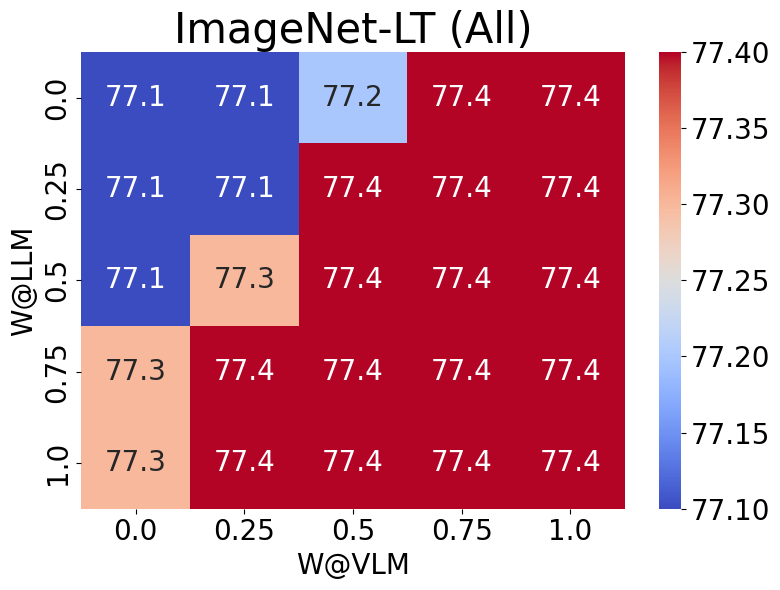
\includegraphics[width=0.49\linewidth]{img/img_avg_r.png} &
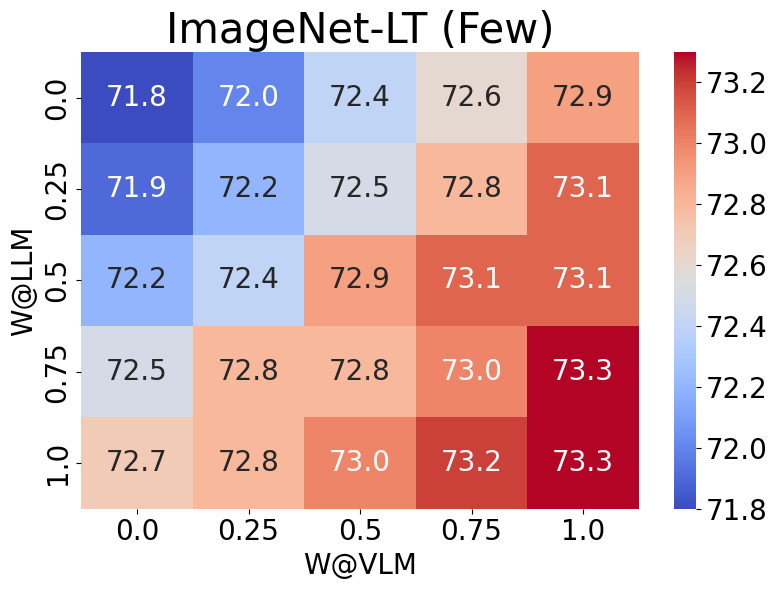
\includegraphics[width=0.49\linewidth]{img/img_few_r.png} \\
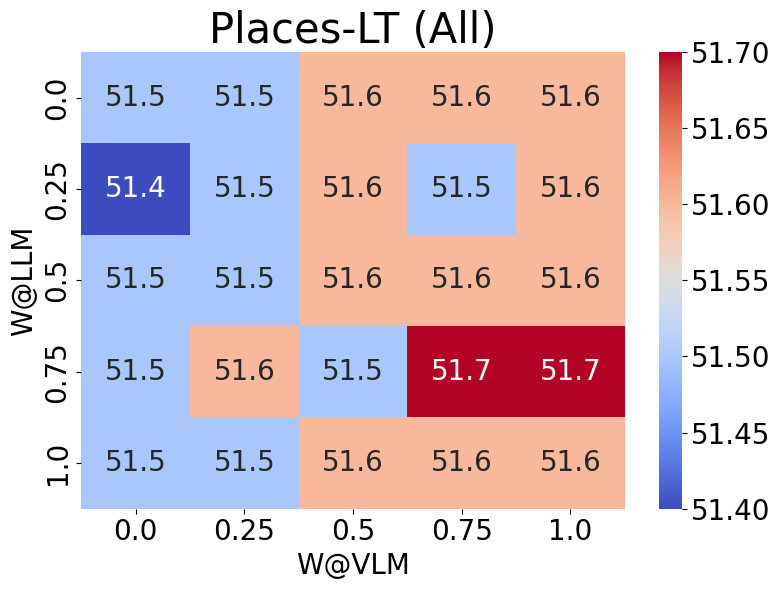
\includegraphics[width=0.49\linewidth]{img/places_avg.png} &
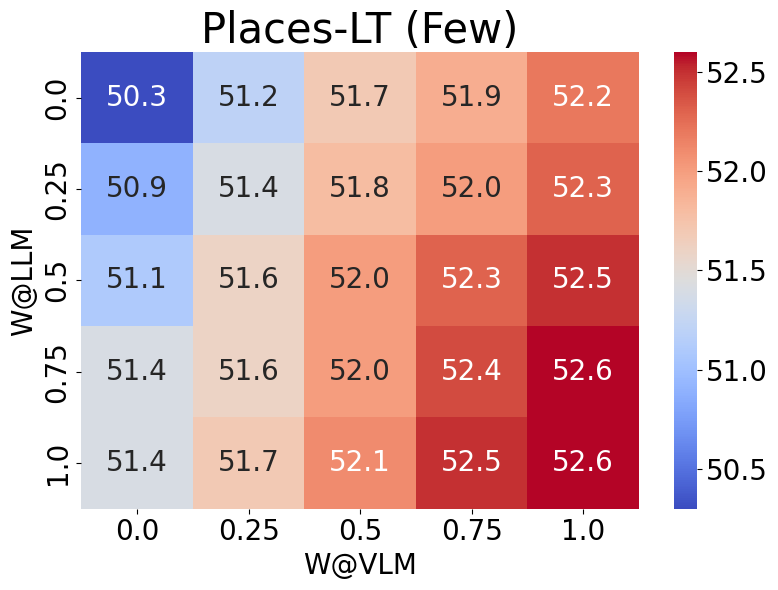
\includegraphics[width=0.49\linewidth]{img/places_few.png}
\end{tabular}
\caption{Sensitivity analysis of CUE with respect to the weighting coefficients $(\lambda_{\text{VLM}}, \lambda_{\text{LLM}})$ on ImageNet-LT and Places-LT (avg/few). 
}
\vspace{-2em}
\label{fig:hyper_sensitivity}
\end{figure}


\subsection{Extension Experiments}
To examine the generality and applicability of CUE, we evaluate it under different adaptation paradigms, including parameter-efficient fine-tuning and from-scratch long-tailed training. 
For fair comparison, we follow the standard settings of prior work for each paradigm.
All experiments in this section are conducted on CIFAR100-LT with an imbalance ratio of IR=100. 
% for consistency and computational efficiency.
% Results on additional datasets are provided in Appendix~\textcolor[HTML]{367DBD}{D}.

\begin{figure*}[!t]
\centering
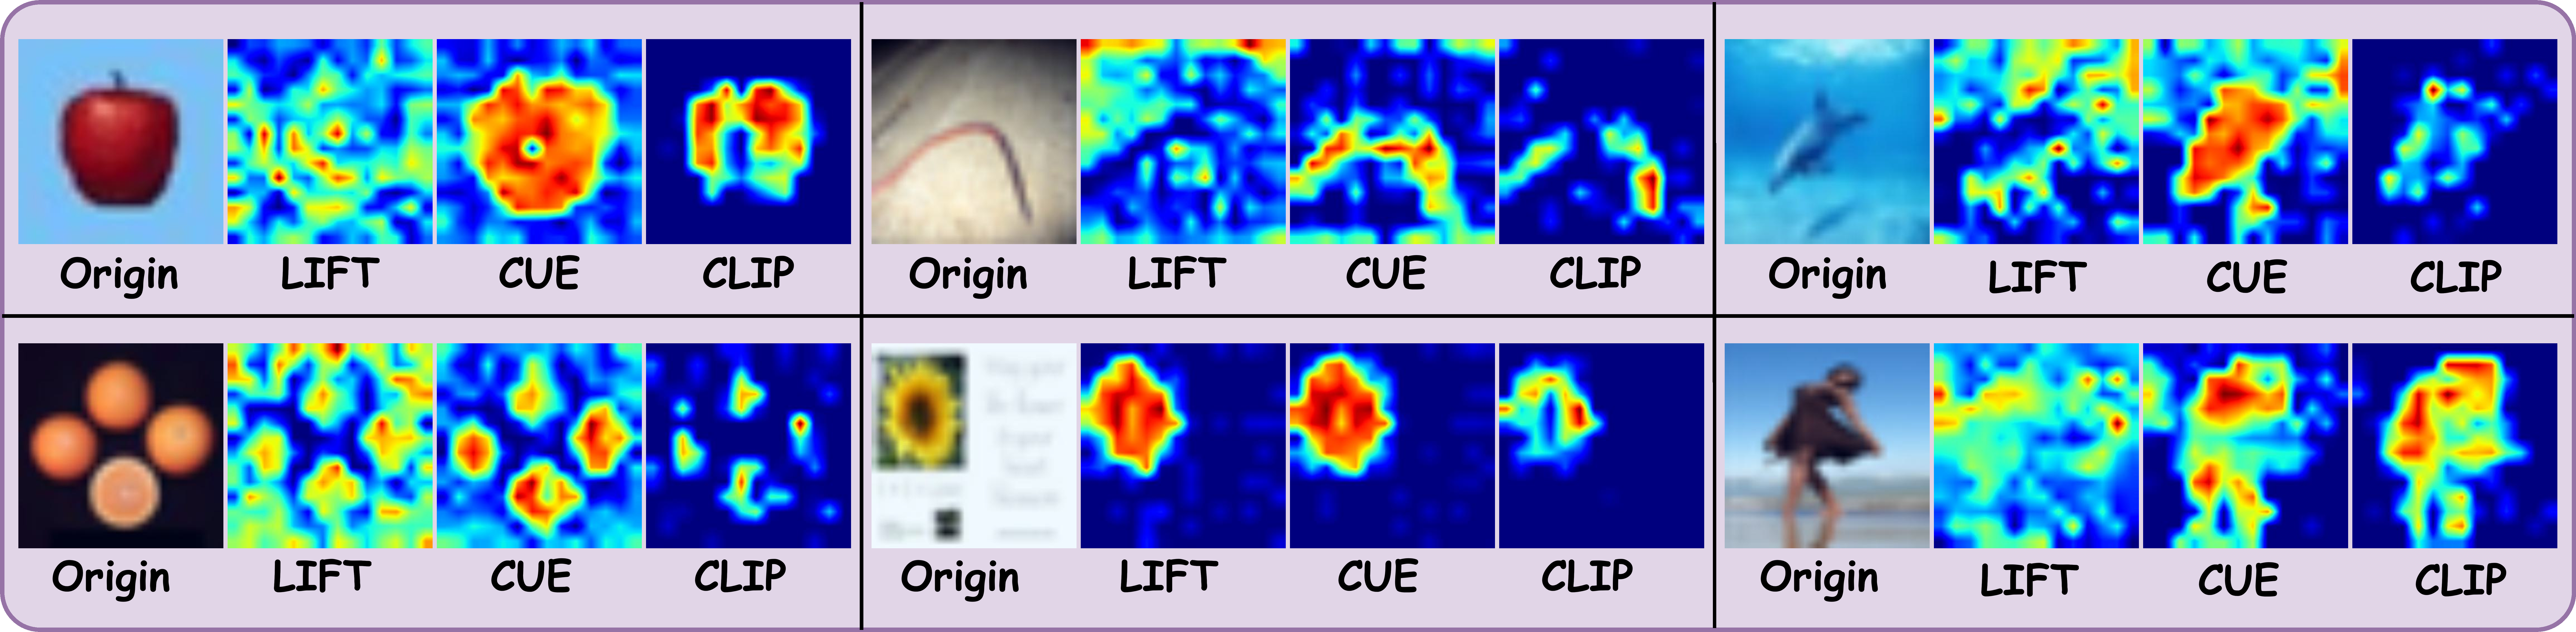
\includegraphics[width=1.0\linewidth]{img/cam_v1.pdf}
\vspace{-1.7em}
\caption{\textbf{Grad-CAM visualization comparing LIFT, CUE and CLIP on several examples}. By sharing related  cues across correlated categories, CUE produces more precise and coherent localization than both LIFT and CLIP.}
\vspace{-1.7em}
\label{fig:gradcam}
\end{figure*}


\label{sec:extension}
% \vspace{0.5em}

\noindent \textbf{Extension to PEFT Methods.}
To examine the generality and flexibility of CUE, we evaluate its integration with several representative parameter-efficient fine-tuning (PEFT) strategies, including LoRA~\cite{hu2022lora}, VPT-shallow~\cite{jia2022visual}, VPT-deep~\cite{jia2022visual}, Adapter~\cite{houlsby2019parameter}, and AdaptFormer~\cite{chen2022adaptformer}.
As reported in Table~\ref{tab:extension_peft}, CUE consistently enhances the performance of all PEFT backbones on CIFAR100-LT (IR=100).
Notably, the gains are particularly pronounced for tail categories, indicating that CUE generalizes well across different parameter-efficient fine-tuning strategies.



\begin{table}[!t]
\centering
\caption{Extension of CUE to different parameter-efficient fine-tuning (PEFT) methods on CIFAR100-IR100. CUE consistently improves performance across various               strategies.}
\label{tab:extension_peft}
\small
\begin{tabular}{l|cccc}
\toprule
\textbf{Method} & \textbf{All} & \textbf{Many} & \textbf{Med.} & \textbf{Few} \\
\midrule
LoRA~\cite{hu2022lora} & 79.1 & 84.0 & \textbf{79.7} & 72.7 \\
+ CUE & \textbf{81.2} & \textbf{84.8} & 79.0 & \textbf{79.8} \\
\midrule
VPT-shallow~\cite{jia2022visual} & 69.7 & \textbf{79.4} & 74.9 & 52.2 \\
+ CUE & \textbf{76.5} & 78.2 & \textbf{75.9} & \textbf{75.2} \\
\midrule
VPT-deep~\cite{jia2022visual} & 78.7 & 81.9 & \textbf{80.0} & 73.5 \\
+ CUE & \textbf{81.0} & \textbf{83.3} & 78.9 & \textbf{80.8} \\
\midrule
Adapter~\cite{houlsby2019parameter} & 79.6 & 83.7 & 80.9 & 73.5 \\
+ CUE & \textbf{82.9} & \textbf{85.8} & 80.9 & \textbf{82.0} \\
\midrule
AdaptFormer~\cite{chen2022adaptformer} & 80.3 & 84.6 & \textbf{81.3} & 74.3 \\
+ CUE & \textbf{82.8} & \textbf{85.7} & 80.5 & \textbf{82.0} \\

\bottomrule
\end{tabular}
\vspace{-1.5em}
\end{table}



% 2. 扩展到from scratch
\vspace{0.5em}

\noindent \textbf{Extension to From-Scratch Training.}
We further verify that CUE is not limited to fine-tuning of pre-trained models but can also be applied to conventional long-tailed training from scratch. 
Since from-scratch training also adopts single-label supervision, the inherent mutual exclusivity still leads to semantic suppression among related categories, resulting in concept confusion. 
Given the plug-and-play nature of CUE, we directly integrate it into several representative from-scratch methods, including DODA~\cite{wang2024kill}, LOS~\cite{sun2025rethinking}, LA~\cite{menon2021longtail}, and ResLT~\cite{cui2022reslt}, without modifying their architectures or optimization pipelines. 
As summarized in Table~\ref{tab:extension_scratch}, all baselines benefit consistently from the inclusion of CUE, demonstrating its generality in mitigating concept confusion across different long-tailed learning paradigms.

\begin{table}[!t]
\centering
\caption{Extension of CUE to from-scratch long-tailed learning methods on CIFAR100-IR100. Consistent improvements demonstrate the plug-and-play nature of our approach.}
\vspace{-0.5em}
\label{tab:extension_scratch}
\small
\begin{tabular}{l|cccc}
\toprule
Method & \textbf{All} & \textbf{Many} & \textbf{Med.} & \textbf{Few} \\
\midrule
DODA~\cite{wang2024kill} &  45.7  &  \textbf{62.1}  &  44.8  &  28.1  \\
+ CUE &  \textbf{47.3}  &  61.8  &  \textbf{45.3}  &  \textbf{33.2}  \\
\midrule
LOS~\cite{sun2025rethinking} &  26.6  &  \textbf{60.7}  &  14.3  &  1.5  \\
+ CUE &  \textbf{31.9}  &  60.2  &  \textbf{25.6}  &  \textbf{6.8}  \\
\midrule
LA~\cite{menon2021longtail} & 42.9 & \textbf{61.3} & 41.0 & 24.1 \\
+ CUE & \textbf{44.1} & 58.8 & \textbf{41.8} & \textbf{29.9} \\
\midrule
ResLT~\cite{cui2022reslt} & 40.4 & \textbf{58.2} & 42.1 & 18.6 \\
+ CUE & \textbf{43.7} & 55.7 & \textbf{44.1} & \textbf{29.6} \\
\bottomrule
\end{tabular}
\vspace{-1.5em}
\end{table}


\subsection{Additional Strengths and Analyses}
\noindent \textbf{(1) Balanced Feature Learning.}
To further understand how CUE improves class-wise balance, we examine the mean number of misclassified samples for \textit{Many}, \textit{Medium}, and \textit{Few} categories, along with the overall balancedness of feature representations. 
Following the balance metric $\beta(V)$ with $\sigma=0.1$ from \cite{kang2020exploring}, we measure feature uniformity based on the pairwise similarity of class-wise accuracies, where a higher $\beta(V)$ indicates more uniform separability across classes. 
As shown in Table~\ref{tab:balance}, CUE consistently achieves fewer misclassifications and higher balancedness scores than LIFT across all three datasets, demonstrating that CUE promotes more balanced and unbiased feature learning by mitigating concept confusion. 
This observation echoes the pattern in Fig.~\ref{fig:motivation2}(a), where baseline models exhibit frequent tail-class misclassifications caused by concept confusion, while CUE effectively alleviates this issue and yields more balanced results.


\begin{table}[!t]
\centering
\caption{Comparison of class-wise balance between LIFT and CUE on three datasets. 
We report mean number of misclassified after fine-tuning for head (\textit{Many}), medium  (\textit{Med.}), and tail (\textit{Few}) classes, 
along with the balancedness score (higer $\beta(V)$ indicates more uniform separability).}
\vspace{-0.5em}
\label{tab:balance}
\footnotesize
\begin{tabular}{l|cccc}
\toprule
\textbf{Method} & \textbf{Many} & \textbf{Med.} & \textbf{Few} & $\beta(V)$\textbf{ ($\uparrow$)} \\
\midrule
\textcolor{gray}{\textbf{CIFAR100-IR100}} & & & & \\
\quad LIFT & 3.1 & \textbf{3.2} & 8.6 & 77.5\% \\
\quad CUE (ours) & \textbf{2.6} & 3.6 & \textbf{4.6} & \textbf{82.9\%} \\[3pt]
\midrule
\textcolor{gray}{\textbf{ImageNet-LT}} & & & & \\
\quad LIFT & 1.9 & 2.6 & 3.7 & 69.7\% \\
\quad CUE (ours) & 1.9 & 2.6 & \textbf{3.2} & \textbf{70.9\%} \\[3pt]
\midrule
\textcolor{gray}{\textbf{Places-LT}} & & & & \\
\quad LIFT & \textbf{5.7} & 5.4 & 7.9 & 60.4\% \\
\quad CUE (ours) & 5.8 & \textbf{5.3} & \textbf{6.9} & \textbf{60.8\%} \\

\bottomrule
\end{tabular}
\vspace{-1.5em}
\end{table}

% gradcam可视化展示 [突出我们的优势]


% \vspace{0.5em}

\noindent \textbf{(2) Improved Feature Localization.}
To further analyze the attention behavior, we visualize Grad-CAM maps for LIFT, CUE, and zero-shot CLIP. As shown in Fig.~\ref{fig:gradcam}, LIFT often focuses on incorrect or irrelevant regions due to concept confusion, while CLIP localizes objects more accurately but lacks domain adaptation to the target dataset. In contrast, CUE inherits the object-centric property of CLIP and enhances it through multi-label cues that encourage related categories to share semantic guidance, resulting in more precise and coherent feature localization.



% \vspace{0.5em}

\noindent \textbf{(3) Effective  Multi-Label Relations.}
% 打标签的相关性示例以及反向实验
% Finally, we present examples of multi-labels derived from the VLM- and LLM-based cues to demonstrate their semantic coherence. The detailed label mappings are provided in Appendix~\textcolor[HTML]{367DBD}{E}. 
To examine the reliability of these cues, we replace the top-$k$ VLM-selected samples with random or last-$k$ ones. As shown in Table~\ref{tab:multi_label_relation}, this substitution leads to a clear degradation in performance, confirming that the proposed cues capture meaningful and semantically consistent relationships rather than spurious correlations.

\begin{table}[!t]
\centering
\caption{Effect of multi-label relation cues on CIFAR100-LT (IR=100). Replacing top-$k$ samples in the VLM-based cue selection with random-$k$ or last-$k$ ones leads to a clear performance drop, verifying the semantic effectiveness of the proposed cues.}
\vspace{-0.5em}
\label{tab:multi_label_relation}
\begin{tabular}{l|cccc}
\toprule
\textbf{Method} & \textbf{All} & \textbf{Many} & \textbf{Med.} & \textbf{Few} \\
\midrule
VLM-based (Top-$k$) & \textbf{82.8} & \textbf{85.7} & 80.8 & \textbf{81.6} \\
VLM-based (random-$k$) & 80.1 & 83.6 & \textbf{81.1} & 75.0 \\
VLM-based (Last-$k$) & 79.5 & 84.0 & 80.9 & 72.5 \\
\bottomrule
\end{tabular}
\vspace{-1.5em}
\end{table}




% ====== drop ============

% CIFAR100 [IR 100 50 10]
% ImageNet-LT
% Places-LT
% inaturalist 2018

% \begin{table*}[!t]
% \centering
% \caption{XXX}
% \footnotesize
% \begin{tabular}{l|cccc|cccc|cccc}
% \toprule
% \multirow{2}{*}{Methods} & \multicolumn{4}{c|}{Places-LT}                                 & \multicolumn{4}{c|}{ImageNet-LT}                               & \multicolumn{4}{c}{iNaturalist}                               \\
%                          & All           & Many          & Med.          & Few           & All           & Many          & Med.          & Few           & All           & Many          & Med.          & Few           \\
% \midrule
% LiVT                     & 40.8          & 48.1          & 40.6          & 27.5          & 60.9          & 73.6          & 56.4          & 41.0          & -         & -             & -             & -          \\
% Decoder~\cite{wang2024exploring}                  & 46.8          & -             & -             & -             & 73.2          & -             & -             & -             & 59.2          & -             & -             & -             \\
% RAC~\cite{long2022retrieval}                      & 47.2          & 48.7          & 48.3          & 41.8          & -             & -             & -             & -             & 80.2          & 75.9          & 80.5          & 81.1          \\
% BALLAD~\cite{ma2021simple}                   & 49.5          & 49.3          & 50.2          & 48.4          & 75.7          & 79.1          & 74.5          & 69.8          & -             & -             & -             & -             \\
% LPT~\cite{dong2023lpt}                   & 50.1         & 49.3          & 52.3          & 46.9          & -          & -         & -          & -         & 76.1             & -             & -             & 79.3             \\
% LIFT~\cite{shi2024long}                     & 51.5          & \textbf{51.3}          & 52.2          & 50.5          & 77.0          & 80.2          & 76.1          & 71.5          & 79.1          & 72.4          & 79.0          & 81.1          \\
% \midrule
% Ours                     & \textbf{51.8} & 51.1 & \textbf{52.5} & \textbf{51.8} & \textbf{77.3} & \textbf{80.3} & \textbf{76.3} & \textbf{72.3} & \textbf{-} & \textbf{-} & \textbf{-} & \textbf{-}  \\
% \bottomrule
% \end{tabular}
% \end{table*}